\section{Data Acquisition}


\subsection{Resources}

\subsection{Public Indexing}

\begin{itemize}
	\item \url{https://github.com/awesomedata/awesome-public-datasets/blob/master/README.rst}
	
	\item \url{https://www.reddit.com/r/datasets/}
	
	
\end{itemize}

\subsection{Notable Database Sites}

\begin{itemize}
	
	% includes leaderboard
	\item \url{https://www.kaggle.com/datasets}
	
	\item \url{https://archive.ics.uci.edu/ml/index.php}
	 
	% US
	\item \url{https://www.data.gov/}
	
	\item \url{https://data.cdc.gov/}
	
	% AU
	\item \url{https://search.data.gov.au/search}
	
	\item \url{https://www.google.com/publicdata/directory}
	
	\item \url{https://data.world/}
	
	% portal search
	\item \url{https://www.opendatasoft.com/a-comprehensive-list-of-all-open-data-portals-around-the-world/?utm_source=general&utm_medium=social&utm_campaign=opendatainception}
	
	\item \url{https://github.com/fivethirtyeight/data}
	
\end{itemize}


\subsection{Data Portal Search}

\subsection{Generating Fake Data}

\textcolor{green}{TODO: generating fake data with SKL}

\textcolor{blue}{make\_blobs}

% {{{datagen_blobs_2dcode}}}
\begin{lstlisting}[style=pyInStyle]
X, y = datagen.make_blobs(centers=4, n_samples=100, n_features=2,cluster_std=1.0,
                          center_box=(-10, 10),
                          random_state=42, shuffle=True)
\end{lstlisting}

% {{{datagen_blobs_2dimg}}}
\begin{figure}
\centering
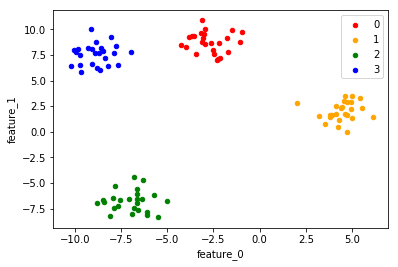
\includegraphics[width=0.65\textwidth]{./sync_imgs/datagen/blobs/2dimg.png}
\label{fig:datagen_blobs_2dimg}
\end{figure}

\textcolor{blue}{Data can also be generated in three (multiple) dimensions}

% {{{datagen_blobs_3dcode}}}
\begin{lstlisting}[style=pyInStyle]
X, y = datagen.make_blobs(centers=4, n_samples=100, n_features=3, random_state=42)
\end{lstlisting}

% {{{datagen_blobs_3dimg}}}
\begin{figure}
\centering
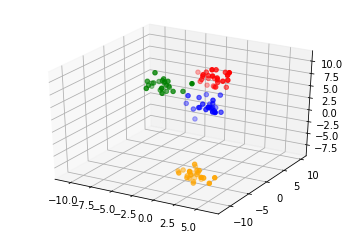
\includegraphics[width=0.65\textwidth]{./sync_imgs/datagen/blobs/3dimg.png}
\label{fig:datagen_blobs_3dimg}
\end{figure}

%\textcolor{blue}{More dataset types can be generated, the documentation can be found at (http://scikit-learn.org/stable/modules/classes.html#module-sklearn.datasets)}


\textcolor{blue}{see \textcolor{red}{local ref?} for more examples on how to generate data}
